% This is the Reed College LaTeX thesis template. Most of the work 
% for the document class was done by Sam Noble (SN), as well as this
% template. Later comments etc. by Ben Salzberg (BTS). Additional
% restructuring and APA support by Jess Youngberg (JY).
% Your comments and suggestions are more than welcome; please email
% them to cusf@reed.edu
%
% See http://web.reed.edu/cis/help/latex.html for help. There are a 
% great bunch of help pages there, with notes on
% getting started, bibtex, etc. Go there and read it if you're not
% already familiar with LaTeX.
%
% Any line that starts with a percent symbol is a comment. 
% They won't show up in the document, and are useful for notes 
% to yourself and explaining commands. 
% Commenting also removes a line from the document; 
% very handy for troubleshooting problems. -BTS

% As far as I know, this follows the requirements laid out in 
% the 2002-2003 Senior Handbook. Ask a librarian to check the 
% document before binding. -SN

%%
%% Preamble
%%
% \documentclass{<something>} must begin each LaTeX document
\documentclass[12pt,twoside]{reedthesis}
% Packages are extensions to the basic LaTeX functions. Whatever you
% want to typeset, there is probably a package out there for it.
% Chemistry (chemtex), screenplays, you name it.
% Check out CTAN to see: http://www.ctan.org/
%%
\usepackage{graphicx,latexsym} 
\usepackage{amssymb,amsthm,amsmath}
\usepackage{longtable,booktabs,setspace} 
\usepackage{subfig}
%\usepackage{chemarr} %% Useful for one reaction arrow, useless if you're not a chem major
\usepackage{url}
\usepackage{natbib}
\usepackage{pdfpages}
% \usepackage{times} % other fonts are available like times, bookman, charter, palatino

\newcommand{\eqn}[1]{\begin{equation}#1\end{equation}}
\newcommand{\eq}[1]{\begin{align}#1\end{align}}
\newcommand{\fig}[2]{\begin{figure}\begin{center}#1\end{center}#2\end{figure}}

\title{Quantum Mechanical Bound States of the Yukawa Potential (or some better title)}
\author{Ellen M. McManis}
% The month and year that you submit your FINAL draft TO THE LIBRARY (May or December)
\date{May 2012}
\division{Mathematics and Natural Sciences}
\advisor{Nelia Mann}
%If you have two advisors for some reason, you can use the following
%\altadvisor{Your Other Advisor}
%%% Remember to use the correct department!
\department{Physics}
% if you're writing a thesis in an interdisciplinary major,
% uncomment the line below and change the text as appropriate.
% check the Senior Handbook if unsure.
%\thedivisionof{The Established Interdisciplinary Committee for}
% if you want the approval page to say "Approved for the Committee",
% uncomment the next line
%\approvedforthe{Committee}

\setlength{\parskip}{0pt}
%%
%% End Preamble
%%
%% The fun begins:
\begin{document}

  \maketitle
  \frontmatter % this stuff will be roman-numbered
  \pagestyle{empty} % this removes page numbers from the frontmatter

% Acknowledgements (Acceptable American spelling) are optional
% So are Acknowledgments (proper English spelling)
    \chapter*{Acknowledgements}
	People. Things. Shep, the dog who is currently keeping me company.

% The preface is optional
% To remove it, comment it out or delete it.
%    \chapter*{Preface}
%	This is an example of a thesis setup to use the reed thesis document class.

    \tableofcontents
% if you want a list of tables, optional
    \listoftables
% if you want a list of figures, also optional
    \listoffigures

% The abstract is not required if you're writing a creative thesis (but aren't they all?)
% If your abstract is longer than a page, there may be a formatting issue.
    \chapter*{Abstract}
	Math and computers and stuff gave me results!
		
%	\chapter*{Dedication}
%	You can have a dedication here if you wish.

  \mainmatter % here the regular arabic numbering starts
  \pagestyle{fancyplain} % turns page numbering back on

%The \introduction command is provided as a convenience.
%if you want special chapter formatting, you'll probably want to avoid using it altogether

    \chapter*{Introduction}
         \addcontentsline{toc}{chapter}{Introduction}
	\chaptermark{Introduction}
	\markboth{Introduction}{Introduction}
	% The three lines above are to make sure that the headers are right, that the intro gets included in the table of contents, and that it doesn't get numbered 1 so that chapter one is 1.

% Double spacing: if you want to double space, or one and a half 
% space, uncomment one of the following lines. You can go back to 
% single spacing with the \singlespacing command.
% \onehalfspacing
% \doublespacing
The Yukawa potential describes a force mediated by a massive particle. It is %argh fuck this part
\eqn{
V(r) = -\frac{C}{r}e^{-r/l}\mbox{,}
}
where $C$ and $l$ are constants. $C$ sets the strength of the force; $l$ acts as a length scale. The exponential term provides an effective cutoff once $r$ gets much larger than $l$, as the exponential term drops off quite rapidly. We are interested in how the bound states of a particle subject to this potential change with these constants. 

A force described by this potential comes from the exchange of massive virtual particles. The length scale, which limits the range at which the force acts, is then related to the mass $m$ by the equation\eqn{
l = \frac{\hbar}{m_{\pi}c}\mbox{.}
}
Both the mass $m$ and the strength of the force $C$ depend on the application of the potential. Most commonly, we use this potential to describe the force between protons and neutrons in an atomic nucleus, where $m$ is the mass of the pion, $m_{\pi} = 140$ MeV/c$^2$.\footnote{I know I'm missing numbers here, will add}

In general, we find the bound states of a system using the time-independent Schr\"odinger wave equation for a particle under the influence of some $V(r)$:
\eqn{
-\frac{\hbar^2}{2\mu}\nabla^2\psi(r,\phi,\theta) + V(r)\psi (r,\phi,\theta) = E \psi(r,\phi,\theta)
\label{eq:TIDSWE-general}
}
and look for solutions which go to zero at infinity.

In this thesis, we are working with a system of two particles moving under the influence of the Yukawa potential (in the atomic case, this would be a deuterium nucleus). To simplify the system, it makes the most sense to express this in spherical coordinates as a reduced mass orbiting a center of mass. This is the form used for the wave equation above. With the Yukawa potential, this equation cannot be solved analytically. However, we can solve the more simple system described by the potential without the exponential term, that is,
\eqn{
 V(r) = -\frac{C}{r}\mbox{.}
 }
This potential is the same form as the Coulomb potential in the hydrogen atom, for which $C = \frac{e^2}{4\pi \epsilon_0}$. While $r << l$, the Yukawa potential should behave similarly to this, because
\begin{equation*}
-\frac{C}{r}e^{-r/l} \approx -\frac{C}{r}
\end{equation*}
in this region. Therefore, we will gain some insight on the Yukawa potential by solving the wave equation for the Coulomb potential.

The solution to this wave equation is well known:
\eqn{
\psi_{l, m_l, n} (r, \theta, \phi) = R_{n,l}(r) Y_{l,m_l}(\theta,\phi)\mbox{.}
}
Here, $l$, $m_l$, and $n$ are quantum numbers. The $Y_{l, m_l}$ are the spherical harmonics. For simplicity, we begin by focusing on states with zero angular momentum, for which the solutions are spherically symmetric. We therefore take $Y_{0,0} = 1/\sqrt{4 \pi}$, leaving us with
\eqn{
\psi_{n, l =0}(r) = R_{n , l= 0}(r) = \frac{1}{\sqrt{4\pi}} e^{-C \mu r / n \hbar^2}\left(\frac{C \mu r}{\hbar^2}\right)^{l} L^{2l + 1 }_{n- l -1} \left(2\frac{C \mu r}{n \hbar^2}\right)
\label{eq:SWE-coulomb}
}
where $L^{2l+1}_{n-l-1}$ is an associated Laguerre polynomial. 

The factor of $e^{-C \mu r / n \hbar^2}$ ensures that the wave function goes to 0 as $r$ goes to infinity, with the $n$ in the denominator controlling how fast that happens. The Laguerre polynomial determines how many nodes the wave function has -- $L^1_{n-1}$ has $n-1$ roots, so the wave function will have that many nodes (figure \ref{fig:wavefunctions}).
\begin{figure}[h]
\centering
\subfloat[]{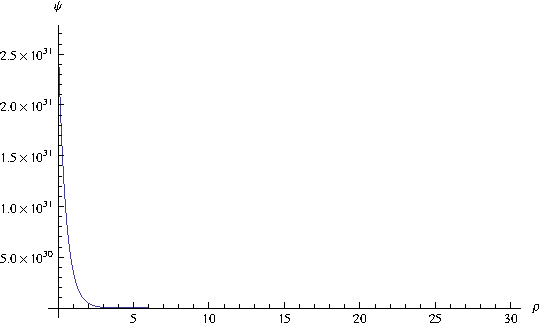
\includegraphics[width=0.3\textwidth]{Figures/ps0}}
\subfloat[]{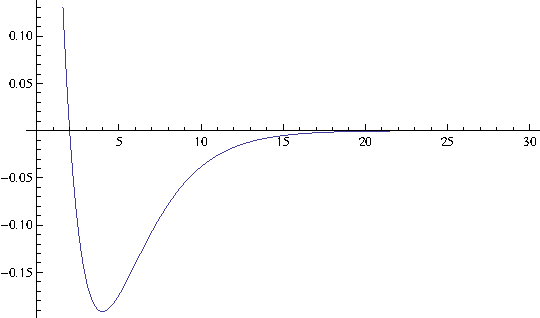
\includegraphics[width=0.3\textwidth]{Figures/ps1}}
\subfloat[]{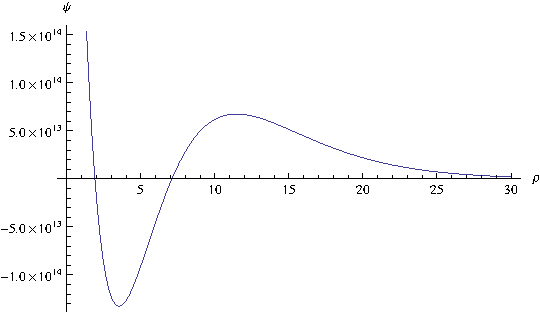
\includegraphics[width=0.3\textwidth]{Figures/ps2}}
\caption{The first three bound states of $\psi(\rho)$ for the Coulomb potential, where $\rho$ is the nondimensionalized radial coordinate. These show the nodes given by the Laguerre polynomials as well as the exponential dieoff of the wave function.}
\label{fig:wavefunctions}
\end{figure}

The energy for the particle described by this wave function is just a function of $n$ (the radial quantum number), and is equal to
\eqn{
E_n = -\frac{\mu C^2}{2\hbar^2 n^2}\mbox{.}
}
All of these functions can be simplified further by introducing a length scale, 
\eqn{
\alpha = \frac{\hbar^2}{C \mu}\mbox{.}
\label{eq:bohrradius}
}
$\alpha$ is a constant with units of length, defined in terms of the other constants of the problem. In hydrogen, this is the Bohr radius, and reduces to the familiar $a_o = \frac{4\pi \epsilon_0 \hbar^2}{\mu e^2}$. Physically, $\alpha$ is the length scale of the exponential term in the ground state of \eqref{eq:SWE-coulomb}. In hydrogen, this determines the size of the smallest electron cloud. As $n$ increases, so do the possible values of $r$, and the particle can be found further and further from the center of mass of the system. This can be seen in figure \ref{fig:hfuncs}, in which $\psi(r)^2$ (the probability density function obtained from $\psi(r)$) is plotted for several values of $n$.
\fig{
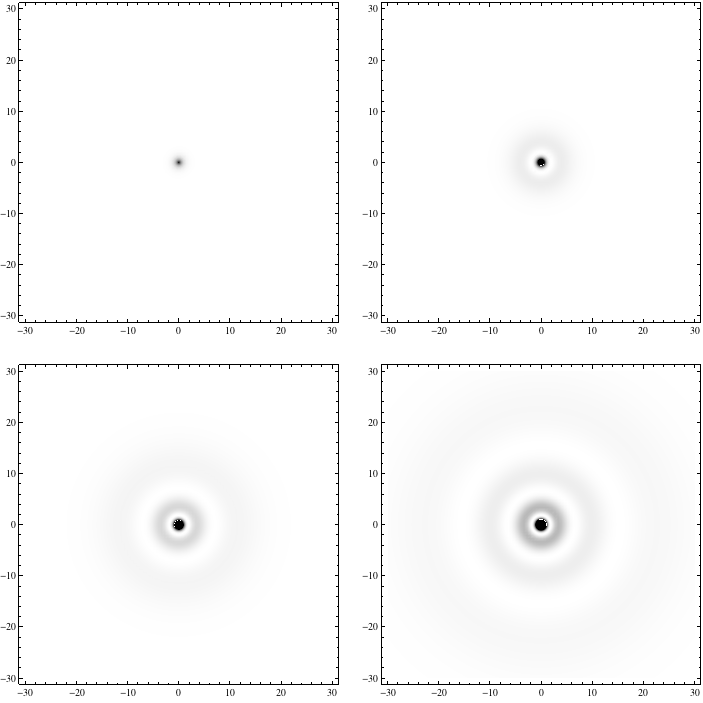
\includegraphics[scale=0.7]{Figures/densityplots}
}{
\caption{The first six spherically symmetric wave functions. This plot shows the probability density, $\psi(\rho)^2$, in spherical coordinates. These plots are all close to the origin, where $\psi$ is large.}
\label{fig:hfuncs}
}
As this happens, $E_n$ gets closer and closer to zero, but never quite reaches it -- there are an infinite number of bound states possible.
%\begin{figure}[h]
%\begin{center}
%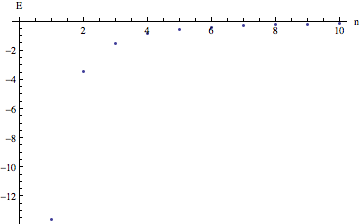
\includegraphics[scale=0.7]{Figures/hydrogenspectrum}
%\end{center}
%\caption{The energies of the first 10 bound states of the electron in the hydrogen atom}
%\label{fig:hspec}
%\end{figure}

Going back to the more-complicated Yukawa potential, the exponential term in the potential means that its range is limited in a way the Coulomb potential's isn't, because $e^{-x}$ drops off much faster than $1/x$. We expect that this will limit the number of bound states as well, to some number whose $r$s are less than $l$.

\clearpage %% starts a new page and stops trying to place floats such as tables and figures

\chapter{Semi-Classical Approximation}
\section{The Bohr Model}
We can again exploit the similarities between the Yukawa potential in deuterium and the Coulomb potential in hydrogen in order to gain some additional insight into the problem before diving into the numerics. We get this from looking at the problem semi-classically, with the Bohr model. The Bohr model is a semi-classical view of the electron orbiting the nucleus in hydrogen. The postulates of the model include the following:
\begin{enumerate}
\item Electrons move in circular orbits around the nucleus under the influence of the Coulomb force. They obey all the laws of classical mechanics.
\item Angular momentum is quantized; $L = n\hbar$ where $n$ is a positive integer.
\item The energy of the electron in an orbit remains constant.
\end{enumerate}

To use these postulates, first, we look at the classical energy of a reduced mass orbiting a center of mass
\eqn{
E = \frac{1}{2}\mu \dot{r}^2+\frac{1}{2}\frac{(n \hbar)^2}{\mu r^2}-V(r)\mbox{.}
\label{eq:classical-energy}
}
We have here used postulate 2 to replace the angular momentum $L$ with $n \hbar$ and multiplied through by $\frac{\alpha}{C}$. 

We can roll the second half of the equation up into an effective potential, producing something of the form $E = KE + PE$. The effective potential $\tilde{V}_{eff}$ is then
\eqn{
\tilde{V}_{eff}(\rho)=\frac{(n \hbar)^2}{2}\frac{1}{\rho^2}+V(\rho)
\label{eq:veff}
}
This equation defines a relationship between the radii of the Bohr orbits, the quantum number $n$, and the energy of the particle in that orbit. 

\section{Application to Coulomb potential}
To make this easier to work with, we use the length scale from \eqref{eq:bohrradius}, the ``Bohr radius'' for this problem. We then use this to nondimensionalize $r$, defining
\begin{equation}
\rho \equiv \frac{r}{\alpha}\mbox{.}
\label{eq:rho}
\end{equation}
Finally, we define a time scale:
\begin{equation}
\beta \equiv \frac{C^2m}{\hbar^3}\mbox{.}
\label{eq:beta}
\end{equation}
We can now substitute these into \eqref{eq:classical-energy} and \eqref{eq:veff} in order to obtain nondimensionalize:
\begin{align}
\frac{\alpha}{C}E &= \tilde{E}= \frac{1}{2}\rho '^2 + \frac{n^2}{2}\frac{1}{\rho^2}-\frac{1}{\rho} \\
\tilde{V}_{eff} &= \frac{n^2}{2}\frac{1}{\rho^2}-\frac{1}{\rho}
\label{eq:veff-nondim}
\end{align}

We can plot the effective potential vs $\rho$ (figure \ref{fig:hveff}). The circular orbits will be at the minimum of this effective potential, where the radius of the particle's orbit is constant.

\fig{
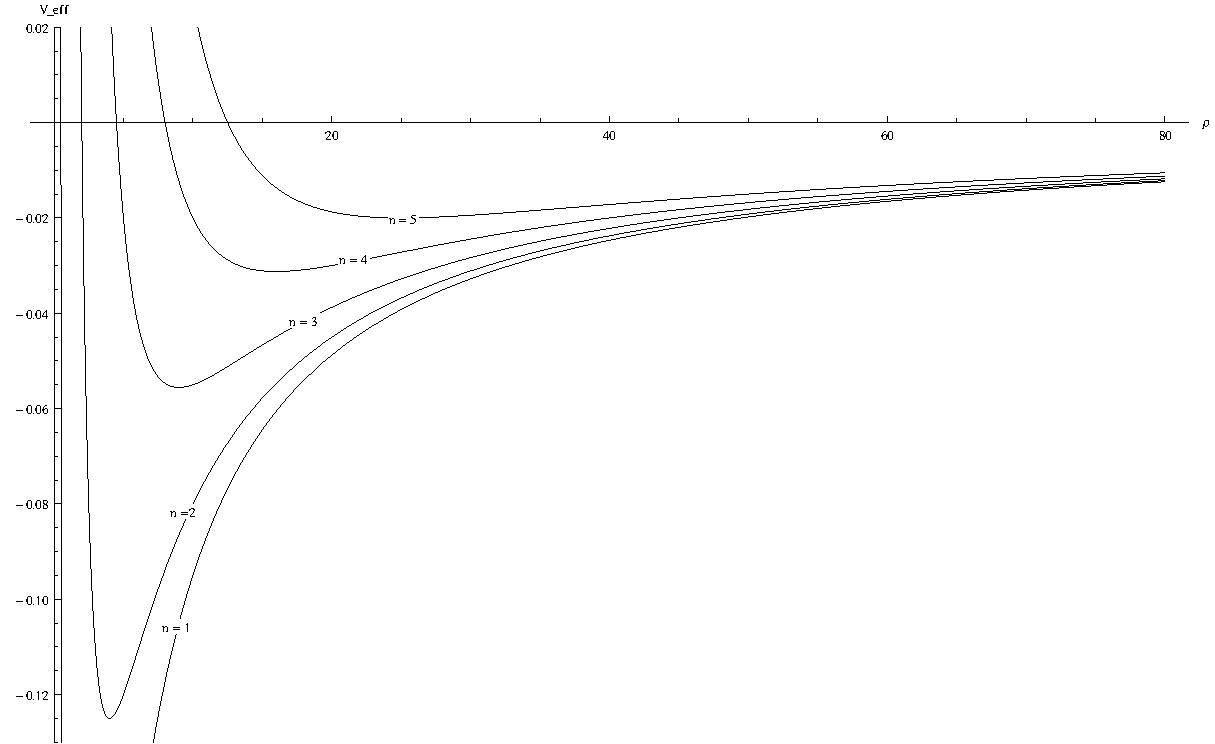
\includegraphics{Figures/hyd_Veff}}
{\label{fig:hveff}
\caption{The effective Coulomb potential. Particles can exist with energies greater than the potential energy, and their trajectories will cover all possible radii at that energy. A particle in a circular orbit, then, must have $E = V_{eff-min}$.}
}

To find the location of this minimum, we differentiate \eqref{eq:veff-nondim} and set the result to $0$:
\begin{align}
0 &= -\frac{n^2}{\rho_0^3} + \frac{1}{\rho_0^2} \\
\rho_0 & = n^2
\label{eq:rho-n}
\end{align}
Fill in the $n$ corresponding to the energy of the desired particle, and there's the radius of its Bohr orbit. For hydrogen, this is perfect -- the semi-classical Bohr model gives exactly the right energy spectrum for the electron, despite the fact that the electron obeys the rules of quantum, not classical mechanics. In other quantum systems, a Bohr approach generally gives a qualitatively reasonable result that's off by a bit quantitatively. For example, when the three-dimensional simple harmonic oscillator is studied, the Bohr method obtains the right form of the solution that differs from the actual solution by an additive constant.

\subsection{Approximating the Yukawa potential with a cutoff}

Returning to the the Yukawa potential, when $r << l$ we expect the $\frac{1}{r}$ term to dominate, and the potential to behave similarly to the Coulomb potential in hydrogen. When $r >> l$, we expect the exponential term to dominate, and the potential to go to zero. As a na\"ive approximation of this behavior, we can consider cutting off the Coulomb potential at $r = l$. In keeping with the nondimensionalization earlier, we define $\lambda \equiv \frac{l}{\alpha}$. Our effective potential is now
\eqn{
\tilde{V}_{eff}(\rho) = \left\{
\begin{array}{lr}
 \frac{n^2}{2}\frac{1}{\rho^2}-\frac{1}{\rho} & : \rho \leq \lambda \\
0 & : \rho > \lambda
\end{array}
\right.
\label{eq:naive}
}

\fig{
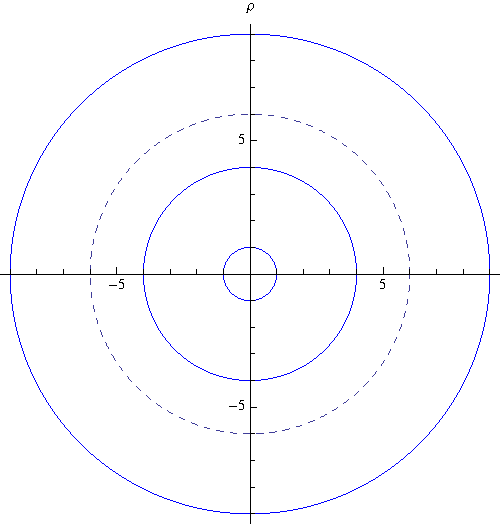
\includegraphics{Figures/cutoff}}
{
\label{fig:cutoff}
\caption{A polar plot of the first three Bohr orbits along with a cutoff at $\lambda = 6$. Because the $n=3$ orbit lies outside the cutoff, it would not be allowed under the na\"ive approximation of the Yukawa potential (equation \eqref{eq:naive})}
}

This cutoff means that the relationship between $\rho$ and $n$ holds while $\rho < \lambda$, but breaks down after, limiting the number of bound states (figure \ref{fig:cutoff}). Any bound state allowed under \eqref{eq:rho-n} for which $\rho$ exceeds $\lambda$ will not exist. Given $\lambda$, then, there will be $\lfloor \sqrt{\lambda} \rfloor$ bound states, and a new bound state will appear when $\sqrt{\lambda} = n$. This gives us a hint of what we should see for the full potential.
\section{Application to Yukawa Potential}
To perform the analysis of the full potential, we look at the graph of its effective potential (figure \ref{fig:yveff}):
\eqn{
\tilde{V}_{eff} = \frac{n^2}{2 \rho^2} - \frac{1}{\rho}e^{-\rho/\lambda}
\label{eq:yveff}
}
 
\fig{
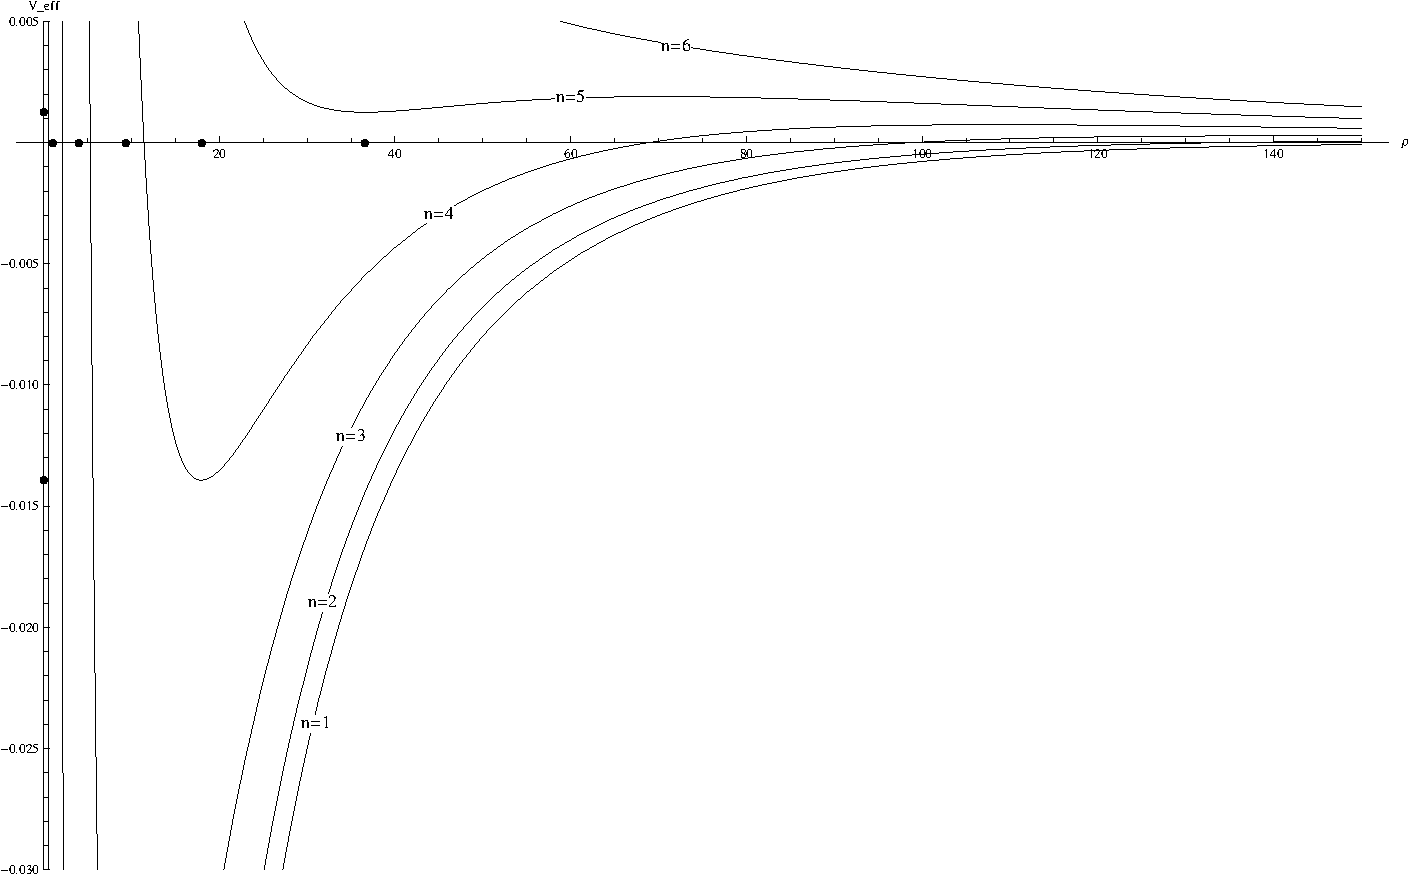
\includegraphics{Figures/yukawa_Veff}}
{
\label{fig:yveff}
\caption{The effective Yukawa potential. All possible bound states occur below $V_{eff} = 0$, which is a limited region, unlike in hydrogen.}
}
 
Just like with hydrogen, above, we can see that bound states exist for $\rho$ where $V_{eff}$ is less than 0, and these bound states have circular orbits at the minimum of $V_{eff}$. Keeping $\alpha$ and $n$ constant, there will then be two critical values of $\lambda$ -- one where $V_{eff}$ has no more stable bound states ($E < 0$), and one where $V_{eff}$ doesn't produce any kind of dip.
\subsection{Stable bound states}
The first of these critical values occurs when the minimum of $V_{eff}$ is 0. We again start by taking the derivative of \eqref{eq:yveff} and setting it to 0, obtaining
\begin{equation}
\frac{dV}{d\rho_0}= -\frac{2n^2}{\rho_0^3} + \frac{2}{\rho_0^2}e^{-\rho_0/\lambda} + \frac{2}{\rho_0 \lambda} e^{-\rho_0/\lambda}
\label{vmin}
\end{equation}
where $\rho_0$ is the value of $\rho$ when $V_{eff}$ is minimized. This equation has no general solution, but we can find one for the specific case where $V_{eff}(\rho_0) = 0$ by solving the equation
\begin{align}
V_{eff}(\rho_0)=0 &= n^2 - 2\rho_0 e^{-\rho_0/\lambda} \\
n^2 &= 2 \rho_0 e^{-\rho_0/\lambda}
\end{align}
and plugging it in to the previous, obtaining
\begin{align}
0 &= -2n^2 + n^2 +n^2 \frac{\rho_0}{\lambda} \\
&= -1 + \frac{\rho_0}{\lambda} \\
\rho_0 &= \lambda \mbox{.}
\end{align}
Plugging this back into the equation for $V_{eff}(\rho_0)$ and forcing $n$ to take an integer value gives us
\begin{equation}
n = \lfloor \sqrt{\frac{2}{e}}\sqrt{\lambda} \rfloor \approx \lfloor 0.857764\sqrt{\lambda} \rfloor
\end{equation}
which is pretty close to the naive $n = \lfloor \sqrt{\lambda} \rfloor$ from above. 
\subsection{Unstable bound states}
For the second critical point, the one where $V_{eff}$ has no minimum, we rewrite \eqref{vmin} to be
\begin{equation}
n^2 = \left( \rho + \frac{\rho^2}{\lambda} \right) e^{-\rho/\lambda}
\end{equation}
The right side of this equation will have some maximum, which will be the last point for which the equation can be solved -- after that, the value of $n^2$ will always be greater than the right side. To find this, we differentiate with respect to $\rho$ and set to 0, obtaining
\begin{align}
0 &= (1+2 \frac{\rho}{\lambda}) - \frac{1}{\lambda}(\rho + \frac{\rho^2}{\lambda}) \\
&= 1 + \frac{\rho}{\lambda} + \frac{\rho^2}{\lambda^2}\mbox{.}
\end{align}
This is a quadratic in $\rho$ and can be solved using the quadratic formula:
\begin{align}
\rho &= \frac{-\frac{1}{\lambda} \pm \sqrt{\left(\frac{1}{\lambda}\right)^2+4\frac{1}{\lambda^2}}}{-\frac{2}{\lambda^2}} \\
&= \frac{\lambda}{2} \mp \frac{\lambda \sqrt{5}}{2}
\end{align}
As $\rho$ is a real physical quantity that can't be negative, we can discard one solution, obtaining
\begin{equation}
\rho = \frac{\lambda}{2}(1+\sqrt{5})
\end{equation}
We can plug this in to \eqref{vmin} to find the relationship between $\lambda$ and $n$:
\begin{align}
n^2 &= \lambda(1+\sqrt{5})\left(\frac{3+\sqrt{5}}{4}\right)e^{-(1+\sqrt{5})/2} \\
n &= \lfloor 0.916494 \sqrt{\lambda} \rfloor \mbox{.}
\end{align}
\section{Summary}
Using the Bohr model to analyze the Yukawa potential suggests that the number of bound states to go up as the square root of $\lambda$.

\clearpage %% starts a new page and stops trying to place floats such as tables and figures

\chapter{Numerical Methods and Spherically Symmetric Results}

\section{The Hamiltonian}

In the previous chapter, we analytically obtained an estimate for the number of bound states allowed by the Yukawa potential given $\lambda$. We now turn our attention to the Schroedinger Wave Equation in order to numerically determine the critical values of $\lambda$ at which a new bound state appears. 

The Wave Equation can be written as
\eqn{
H \psi = E\psi
\label{eq:hamiltonian}
}
where $H$ is the Hamiltonian operator, $H =-\frac{\hbar^2}{2m}\nabla^2 +V$.  Because we are focusing on spherically symmetric bound states, we are only concerned about the $r$ component of the $\nabla$ operator. Equation \eqref{eq:hamiltonian} then becomes
\eqn{
H = -\frac{\hbar^2}{2m} \left[\frac{1}{r^2}\frac{d}{dr}\left(r^2 \frac{d}{dr}\right)\right] - \frac{C}{r}e^{-r/l}\mbox{,}
}
plugging in the Yukawa potential for $V$.

Using the same nondimensionalizations as in last chapter, we rewrite this as 
\eqn{
H=\frac{C}{2\alpha}\tilde{H} = \frac{C}{2\alpha} \left[- \frac{1}{\rho^2}\frac{d}{d\rho}\left(\rho^2\frac{d}{d\rho}\right) - \frac{2}{\rho}e^{-\rho/\lambda}\right]\mbox{.}
\label{eq:hnondim}
}
The constant out front is the same one we pulled when we nondimensionalized the energy of the system, which allows us to restate \eqref{eq:hamiltonian} as
\eqn{
\tilde{H}\psi = \tilde{E}\psi\mbox{.}
}
To simplify, we can substitute \footnote{I should have a cite here.} $u(\rho)=\rho \phi(\rho)$ into the expression in \eqref{eq:hnondim}. This gives us a much neater Hamiltonian, and our differential equation is now
\eqn{
-\frac{d^2 u }{d \rho^2} - \frac{2}{\rho}e^{-\rho/\lambda}u = E u\mbox{.}
\label{eq:hamiltonianfinal}
}

\section{Numerics: The Finite Difference Method}
The finite difference method transforms a differential equation into a matrix problem. It does this by approximating the first and second derivatives of a function on a discrete grid of points $x_n$ which are a distance $\Delta x$ apart. Using the concept of the derivative as the slope of the tangent line to some point, we can write
\eqn{
u'(\rho_n) + O(\Delta{\rho}^2) = \frac{u(\rho_n + \Delta \rho) - u(\rho_n - \Delta \rho)}{2 \Delta \rho}
\label{fdifference}
}
\eqn{
u''(\rho_n) + O(\Delta{\rho}^2) = \frac{u(\rho_n + \Delta \rho) - 2 u(\rho_n) + u(\rho_n - \Delta \rho)}{\Delta \rho^2}
\label{f2difference}
}
We can rewrite $u(\rho_n)$ as $u_n$ and apply \eqref{f2difference} to our differential equation in \eqref{eq:hamiltonianfinal}, obtaining
\eqn{
-u_{n-1}\frac{1}{\Delta \rho^2} - u_n\left(\frac{2} {\Delta \rho^2} -  \frac{2}{\rho_n}e^{-\rho_n/\lambda} \right) - u_{n-1}\frac{1}{\Delta \rho^2}  = E u_n\mbox{.}
\label{eq:hamiltonian-disc}
}
This is runs from $u_1$ to some $u_N$. For the interior points, there are no concerns, but at the beginning we require a $u_0$ and at the end we need a $u_{N+1}$ in order to satisfy \eqref{eq:hamiltonian-disc}. For our problem, $u_0$ is 0 (because $0 * \psi(0) = 0$), and we also require that $u_{N+1}$ be 0 in order to satisfy the condition that bound states go to 0 at infinity. We therefore note this point as $u(\rho_{\infty})$. 

We now construct a hamiltonian matrix using \eqref{eq:hamiltonian-disc}. The matrix will have entries on the off diagonal and diagonal and nowhere else:
\begin{equation*}H = \left(
\begin{array}{cccccc}
\frac{2} {\Delta \rho^2} -  \frac{2}{\rho_1}e^{-\rho_1/\lambda} & -\frac{1}{\Delta \rho^2} &  0 & 0 & 0 & 0 \\
-\frac{1}{\Delta \rho^2} & \frac{2} {\Delta \rho^2} -  \frac{2}{\rho_2}e^{-\rho_2/\lambda} &  -\frac{1}{\Delta \rho^2}  & 0 & 0 & 0 \\
0 &  -\frac{1}{\Delta \rho^2} & \frac{2} {\Delta \rho^2} -  \frac{2}{\rho_3}e^{-\rho_3/\lambda} &  -\frac{1}{\Delta \rho^2}  & 0 & 0 \\
 .&  . &.  &. & .& .  \\
 .& . & . & .& .&  . \\
0 & 0 &  0 & 0&  -\frac{1}{\Delta \rho^2} & \frac{2} {\Delta \rho^2} -  \frac{2}{\rho_N}e^{-\rho_N/\lambda}   \\
\end{array}
\right)
\end{equation*}
The eigenvectors of this matrix will be the wave functions $u(\rho_n)$, and the eigenvalues will be the energies of those wave functions.

Using this, we can now see what our wave functions actually look like. For bound states where $n^2 << \lambda$, we find that the bound states look very similar to hydrogen, with the exception of sign (figure \ref{fig:hyd-yukawa}).
\begin{figure}[h]
\centering
\subfloat[]{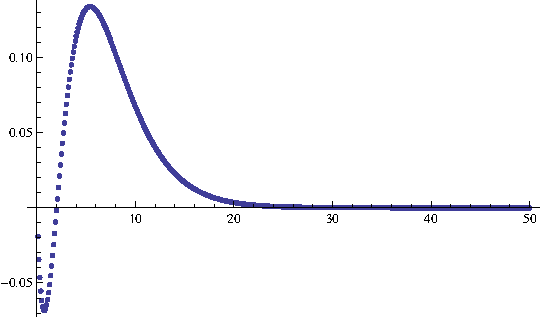
\includegraphics[width=0.5\textwidth]{Figures/n2yukawa}}
\subfloat[]{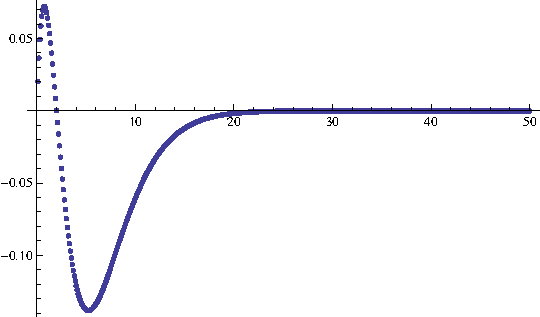
\includegraphics[width=0.5\textwidth]{Figures/n2hyd}}
\caption{The $n = 2$ bound states for the Yukawa potential (left) and Coulomb potential (right). Both were calculated using my finite difference Hamiltonian. For the Yukawa potential, $\lambda = 12.9$, and for both, $\rho_{\infty} = 20*12.9 = 258$. The plot only extends out to $\rho = 50$ in order to see the earlier behavior; the function is remains 0 further out.}
\label{fig:hyd-yukawa}
\end{figure}
As $\lambda$ increases and more bound states are possible, the wave functions get more interesting, as in figure \ref{fig:largebound}.
\begin{figure}[h]
\centering
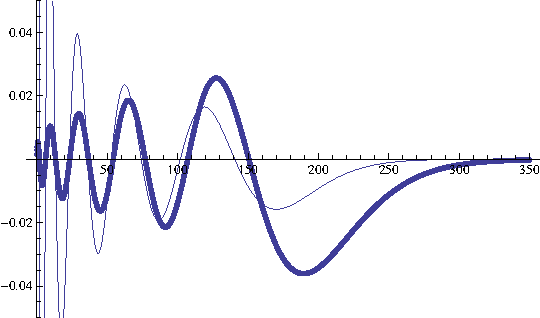
\includegraphics{Figures/hyukawa10}
\caption{The $n=10$ bound state at $\lambda = 200$. The $n=10$ Coulomb wave function is shown as well. While they start out close together, the Coulomb wave function goes to zero faster and the wave functions diverge a bit towards the end. This plot shows the whole range where anything interesting is going on -- again, the function has gone to 0 and will stay there.}
\label{fig:largebound}
\end{figure}
\section{Finding Critical Values of Lambda}

\section{Estimating errors}
Requirements for $\rho_{inf}$ and $\Delta \rho$

Asymptotic behaviors

\section{Results and fit}
Pictures!

Discussion of fit options:

log log plot

quadtratic fit

%\clearpage %% starts a new page and stops trying to place floats such as tables and figures

%
%
%\chapter*{Conclusion}
%         \addcontentsline{toc}{chapter}{Conclusion}
%	\chaptermark{Conclusion}
%	\markboth{Conclusion}{Conclusion}
%	\setcounter{chapter}{4}
%	\setcounter{section}{0}
%	
%
%If you feel it necessary to include an appendix, it goes here.
\appendix
\chapter{Numerical Methods}
To actually locate the critical values of lambda, we need to find the place where a new bound state appears. Numerically, this looks like a new negative eigenvalue in our list, which suggests we approach the problem with rootfinding. Our function has a ``zero'' whenever the number of negative eigenvalues increases.

The rootfinder actually used was a recursive bisection routine:
\begin{verbatim}
Bisect (low, high, delta):
    mid = low + (high-low)/2
    If (high - low < delta)
       Return mid
    Else if negs(low) < negs(mid)
        Bisect(low, mid)
    Else 
        Bisect(mid, high)
\end{verbatim}
We use a $\delta$ here instead of the usual $\epsilon$ because we are interested in minimizing uncertainty in $\lambda$, not the function we are performing rootfinding on. There either is or isn't an additional eigenvalue, so $\epsilon$ has little meaning and would be complicated to compute.

To find the ranges to bisect, we modify the rootfinder so it keeps bisecting as long as there is a zero in one of the ranges, and returns a list of points instead of just one. For efficiency's sake, this calculation is run at a low $\rho_{\infty}$, and a range is returned instead of a single point. That range can then be bisected more thoroughly in order to identify the most likely point. 

The function doing the actual work is just Mathematica's Eigenvalues[ ]. Because our Hamiltonian matrix only has entries on the diagonal and off-diagonals, we can define it as a SparseArray to speed up calculation. 

\subsection{Parallelization}

Finding a single $\lambda_{c}$ takes quite a bit of time -- it's expensive to find the eigenvalues of a large matrix, even such a sparse one as ours. We would like to study a wide range of $\lambda$s, and the computation begins to look prohibitively expensive.

This is where the cluster comes in. Mathematica has easy build in parallelization methods, and once we have ranges to bisect, each $\lambda_{c}$ calculation is independent from all the others. Distributing these calculations among multiple cores speeds the process up considerably, making this thesis possible.\footnote{I put this in because it felt like it should be in here, but have really no idea what to say.}
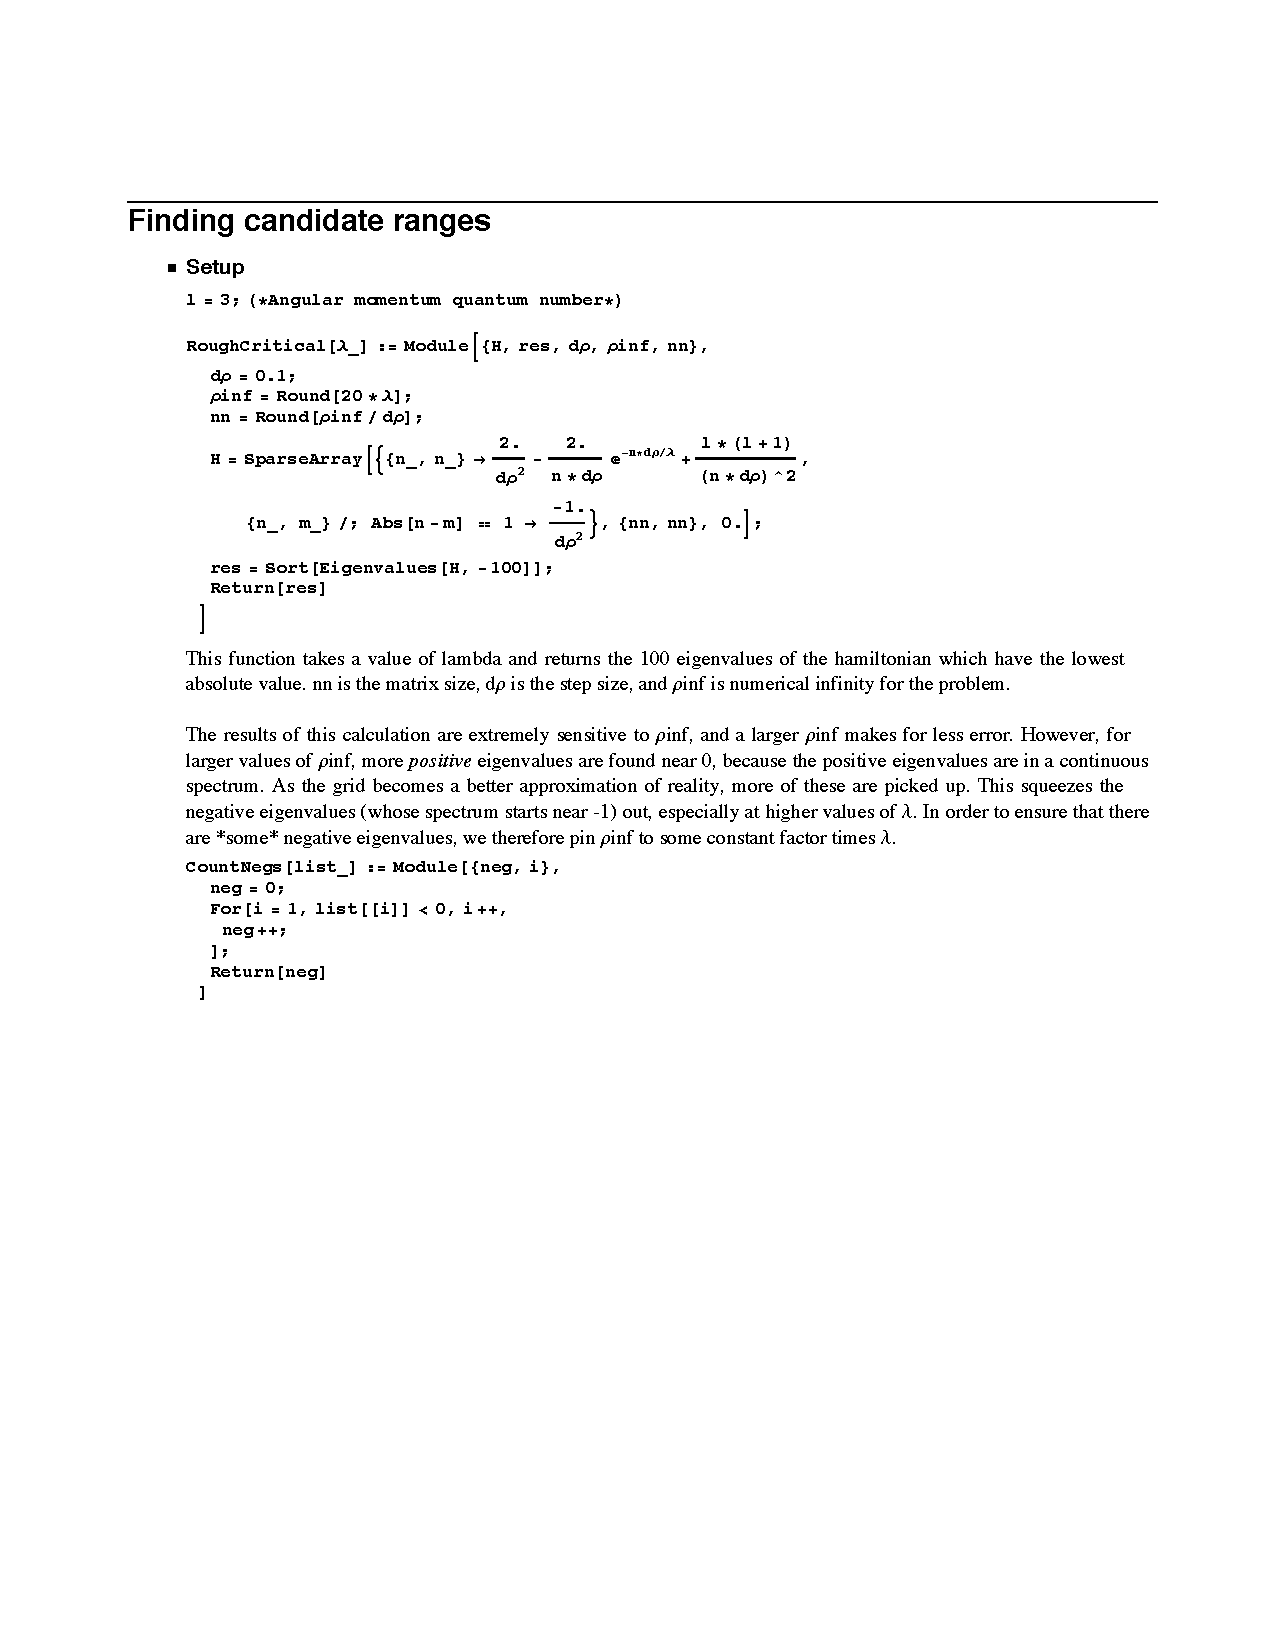
\includepdf{find_lcs.pdf}

%      \chapter{The Second Appendix, for Fun}
%
%
%%This is where endnotes are supposed to go, if you have them.
%%I have no idea how endnotes work with LaTeX.
%
\backmatter % backmatter makes the index and bibliography appear properly in the t.o.c...
%
% Make my bibliography be called "Bibliography" and not "References" (or "Works Cited" or...):
%% \renewcommand{\bibname}{Works Cited}

 \bibliographystyle{plain}
%FIXME: should be apsrev.
  
% there are a variety of styles available; 
%% replace ``plainnat'' with the style of choice. You can refer to files in the bsts or APA 
%% subfolder, e.g. 
%% \bibliographystyle{APA/apa-good}  % or
%% \bibliographystyle{bsts/mla-good} 
%
%% if you're using bibtex, the next line forces every entry in the bibtex file to be included
%% in your bibliography, regardless of whether or not you've cited it in the thesis.
   \nocite{*}
   \bibliography{em_thesis}

% Finally, an index would go here... but it is also optional.
\end{document}
